%-----------------------------------------------------------------------------%
\chapter{\babTiga}
%-----------------------------------------------------------------------------%
Bab ketiga ini menjelaskan tentang rancangan dan metodologi yang penulis lakukan dalam penelitian ini. Sub-bab 3.1 menjelaskan mengenai tahapan penelitian yang akan penulis lakukan. Sub-bab 3.2 menjelaskan bagaimana persiapan data, model, dan metode yang akan dilakukan pada penelitian ini. Sub-bab 3.3 menjelaskan pelatihan model dan alur eksperimen yang dilakukan. Sub-bab 3.4 lalu menjelaskan metrik umum yang digunakan setiap metode dan metrik khusus yang digunakan untuk setiap metode.

%-----------------------------------------------------------------------------%
\section{Pembuka}
%-----------------------------------------------------------------------------%

Sebagai pembuka dari bagian metodologi ini, penelitian ini ditujukan untuk mengetahui apakah performa sistem tanya jawab berbahasa Indonesia akan lebih baik dengan memanfaatkan NLI dan jenis-jenis pertanyaan apa saja yang lebih baik dengan memanfaatkan NLI. Bab metodologi ini akan berfokus kepada gambaran umum dari penelitian ini.

%-----------------------------------------------------------------------------%
\section{Tahapan Penelitian}
%-----------------------------------------------------------------------------%
Pada sub-bab ini, akan dijelaskan mengenai tahapan penelitian yang penulis gunakan pada penelitian ini. Tahapan penelitian yang penulis lakukan adalah sebagai berikut:

\begin{itemize}
    
    \item \textbf{Persiapan data, model, dan metode}: Pada tahap ini penulis melakukan pencarian untuk memilih data, model, dan metode eksperimen apa saja yang akan digunakan dalam penelitian ini. Tahap ini meliputi pemilihan data dan model yang akan digunakan untuk tiap metode dan penjelasan metode yang dipakai untuk penelitian. Kemudian, untuk metode penelitian, penulis memutuskan untuk menggunakan tiga metode eksperimen, yaitu: \emph{intermediate-task transfer learning}, \emph{task recasting} dengan IndoNLI sebagai verifikator, dan \emph{task recasting} dengan IndoNLI sebagai penghasil jawaban. Hasil dari tahap ini adalah data yang akan digunakan pada tahap selanjutnya.

    \item \textbf{Eksplorasi \emph{dataset} (EDA)}: Pada tahap ini penulis melakukan eksplorasi dari \emph{dataset} sistem tanya jawab yang telah dipilih sebelumnya. Eksplorasi \emph{dataset} (EDA) dilakukan dengan bertujuan untuk mengerti karakteristik dari suatu \emph{dataset} sistem tanya jawab yang sedang diproses.
    
    \item \textbf{Pelatihan model dan eksperimen}: Pada tahap ini penulis melakukan pelatihan model dan eksperimen-eksperimen berdasarkan data, model, dan metode yang sudah dipilih pada tahap sebelumnya. Tahap ini meliputi pelatihan model yang akan digunakan untuk tiap metode. Hasil dari tahap ini adalah model yang sudah dilatih berdasarkan metode yang telah dipilih yang menghasilkan hasil eksperimen untuk dilakukan analisis pada tahap berikutnya.

    \item \textbf{Evaluasi dan analisis hasil}: Pada tahap ini penulis melakukan evaluasi dan analisis berdasarkan hasil yang sudah didapatkan pada tahap sebelumnya. Tahap ini meliputi pemilihan metrik evaluasi yang digunakan untuk setiap metode eksperimen penelitian.

\end{itemize}

%-----------------------------------------------------------------------------%
\section{Persiapan Data, Model, dan Metode}
%-----------------------------------------------------------------------------%
Pada sub-bab ini, akan dijelaskan mengenai data, model, dan metode yang penulis gunakan pada eksperimen-eksperimen pada penelitian ini. 

%-----------------------------------------------------------------------------%
\subsection{Data dan Model}
%-----------------------------------------------------------------------------%
Data yang penulis gunakan dapat terbagi menjadi dua bagian, data NLI dan data sistem tanya jawab. Untuk data NLI, penulis hanya menggunakan satu \emph{dataset}, yaitu: \emph{dataset} IndoNLI \citep{mahendra-etal-2021-indonli}. Alasan menggunakan \emph{dataset} ini adalah: karena topik utama penelitian ini adalah melanjutkan topik penelitian \citet{mahendra-etal-2021-indonli} terkait pemanfaatan \emph{dataset} IndoNLI pada beragam tugas (\emph{task}) bidang NLP, salah satunya adalah sistem tanya jawab (\emph{question answering}). Kemudian, untuk data sistem tanya jawab, penulis menggunakan tiga \emph{dataset} sebagai tolak ukur (\emph{benchmark}) dari evaluasi sistem tanya jawab yang penulis rancang, yaitu: \emph{dataset} SQuAD-ID \citep{muis2020sequencetosequence}, TyDi-QA-ID \citep{cahyawijaya-etal-2021-indonlg}, IDK-MRC \citep{putri-oh-2022-idk}. Alasan menggunakan ketiga \emph{dataset} ini adalah: karena menurut penulis, ketiga \emph{dataset} ini merupakan \emph{dataset} terbaik untuk dijadikan tolak ukur (\emph{benchmark}) sistem tanya jawab berbahasa Indonesia. Penggunaan tiga \emph{dataset} sekaligus juga penulis tujukan agar sistem tanya jawab dapat menangkap pola-pola variasi beragam \emph{dataset} sistem tanya jawab, sehingga sistem tanya jawab buatan penulis berhasil menggeneralisasikan pola-pola tersebut untuk menghasilkan prediksi jawaban yang lebih \emph{robust}.

%-----------------------------------------------------------------------------%
\subsection{Metode Eksperimen}
%-----------------------------------------------------------------------------%
Pada sub-bab ini, akan dijelaskan beberapa metode yang penulis pilih, yaitu: \emph{intermediate-task transfer learning}, \emph{task recasting} dengan IndoNLI sebagai verifikator jawaban, dan \emph{task recasting} dengan IndoNLI sebagai penghasil jawaban. 

%-----------------------------------------------------------------------------%
\subsubsection{\emph{Intermediate-Task Transfer Learning}}
%-----------------------------------------------------------------------------%
Pada tahapan eksperimen ini, penulis menggunakan metode yang persis digunakan oleh \citep{pruksachatkun-etal-2020-intermediate}, yaitu dengan memecah tugasnya menjadi dua, yaitu: \emph{intermediate task} dan \emph{target task}. Pada penelitian ini, \emph{intermediate task} yang dipilih adalah \emph{sequence classification task} dengan menggunakan \emph{dataset} IndoNLI, dan \emph{target task} yang dipilih adalah \emph{question answering task} dengan menggunakan \emph{dataset} SQuAD-ID, TyDi-QA-ID, dan IDK-MRC. Untuk alur eksperimen tahap ini, akan dijelaskan pada sub-bab selanjutnya.

%-----------------------------------------------------------------------------%
\subsubsection{\emph{Task Recasting} dengan IndoNLI sebagai verifikator}
%-----------------------------------------------------------------------------%
Pada tahapan eksperimen ini, penulis menggunakan metode yang persis digunakan oleh \citep{chen-etal-2021-nli-models}, yaitu dengan melakukan penyaringan (\emph{filtering}) prediksi jawaban dengan parameter hasil label NLI-nya. Pada penelitian ini, prediksi jawaban oleh model \emph{question answering} tidak diganggu sama sekali, setelah prediksi jawaban didapatkan, baru dilakukan penyaringan (\emph{filtering}) prediksi jawabannya. Untuk alur eksperimen tahap ini, akan dijelaskan pada sub-bab selanjutnya. 

%-----------------------------------------------------------------------------%
\subsubsection{\emph{Task Recasting} dengan IndoNLI sebagai penghasil jawaban}
%-----------------------------------------------------------------------------%
\todo

%-----------------------------------------------------------------------------%
\section{Eksplorasi \emph{dataset} (EDA)}
%-----------------------------------------------------------------------------%
Pada sub-bab ini, akan dijelaskan mengenai eksplorasi \emph{dataset} (EDA) sistem tanya jawab yang telah dipilih sebelumnya. Eksplorasi yang penulis lakukan sama persis dengan apa yang telah dilakukan \citet{nguyen-etal-2020-vietnamese} dan \citet{rajpurkar-etal-2016-squad} pada tahapan ekplorasi \emph{dataset machine reading comprehension} untuk bahasa Vietnam. Ada beberapa bagian yang penulis jadikan bahan eksplorasi, antara lain:

\begin{itemize}

    \item \emph{Overview Statistics}

        \begin{itemize}
            \item Banyaknya artikel.
            \item Banyaknya konteks.
            \item Banyaknya pertanyaan.
            \item Banyaknya jawaban yang eksis.
            \item Banyaknya jawaban yang tidak eksis.
            \item Rata-rata panjang kata dari konteks.
            \item Rata-rata panjang kata dari pertanyaan.
            \item Rata-rata panjang kata dari jawaban.
            \item \emph{Vocabulary size}.
        \end{itemize}

    \item \emph{Length-based analysis}

        \begin{itemize}
            \item Rincian distribusi panjang kata dari konteks.
            \item Rincian distribusi panjang kata dari pertanyaan.
            \item Rincian distribusi panjang kata dari jawaban.
        \end{itemize}
        
    \item \emph{Type-based analysis}

        \begin{itemize}
            \item \emph{Question type}.
            \item \emph{Reasoning type}.
            \item \emph{Answer type}.
        \end{itemize}

\end{itemize}

Properti-properti di atas yang akan menjadi bahan evaluasi dan analisis penelitian ini yang telah tertuang pada \hyperref[sec:rumusanMasalah]{rumusan masalah} dan \hyperref[sec:tujuanPenelitian]{tujuan penelitian} yang telah dituliskan di \hyperref[bab:1]{bab 1} di atas. Penggunaan properti-properti di atas ditujukan untuk mendalami dan menambah wawasan terkait \emph{dataset} sistem tanya jawab.


%-----------------------------------------------------------------------------%
\section{Pelatihan Model dan Eksperimen}
%-----------------------------------------------------------------------------%
Pada sub-bab ini, akan dijelaskan mengenai pelatihan model dan eksperimen yang penulis lakukan pada pada penelitian ini. 

%-----------------------------------------------------------------------------%
\subsection{\emph{Intermediate-Task Transfer Learning}}
%-----------------------------------------------------------------------------%

\begin{figure}[h]
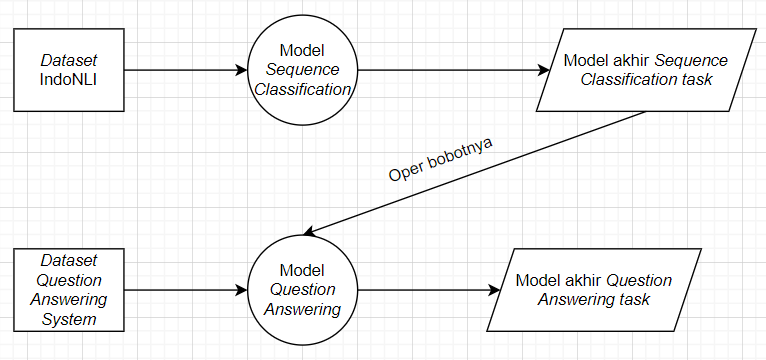
\includegraphics[width=\linewidth]{assets/pics/alur1.png}
\centering
\caption{Visualisasi grafik pada metode \emph{intermediate-task transfer learning}.}
\end{figure}

Alur penelitian tahapan \emph{intermediate-task transfer learning} yang penulis lakukan adalah sebagai berikut:

\begin{itemize}
    
    \item Model-model yang telah dipilih sebelumnya, akan dilatih terlebih dahulu pada \emph{task} \emph{sequence classification} sebagai \emph{intermediate task}-nya.

    \item Setelah model selesai dilatih pada \emph{task} \emph{sequence classification}, kemudian bobot (\emph{weight}) dari hasil latih tersebut disimpan terlebih dahulu.

    \item Kemudian, model-model baru akan diinisiasikan dengan \emph{task} \emph{question answering} sebagai \emph{target task}-nya.

    \item Namun, bobot model untuk \emph{task} \emph{question answering} didapatkan dari bobot model \emph{task} \emph{sequence classification} yang sebelumnya disimpan. Disini, penulis membuat dua alur, pertama, apakah bobot dari  \emph{task} \emph{sequence classification} akan dilatih ulang semua \emph{layer}-nya atau hanya akan dilatih ulang pada \emph{layer} klasifier-nya saja \citep{lee2019elsa}.

\end{itemize}

%-----------------------------------------------------------------------------%
\subsection{\emph{Task Recasting} dengan IndoNLI sebagai verifikator}
%-----------------------------------------------------------------------------%

\begin{figure}[h]
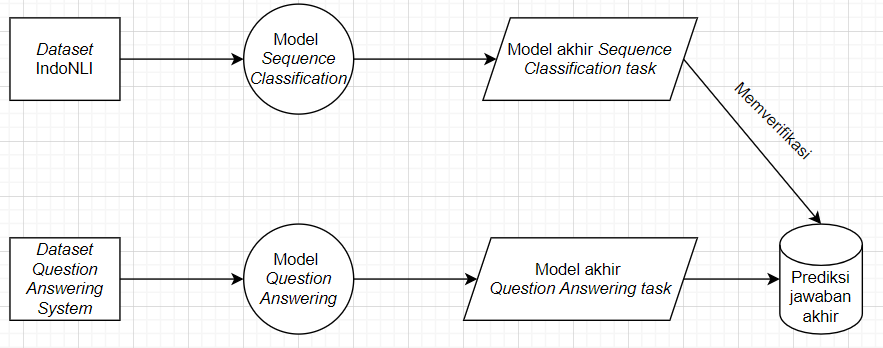
\includegraphics[width=\linewidth]{assets/pics/alur2.png}
\centering
\caption{Visualisasi grafik pada metode \emph{task recasting} dengan IndoNLI sebagai verifikator.}
\end{figure}

Alur penelitian tahapan \emph{task} Recasting dengan IndoNLI sebagai verifikator yang penulis lakukan adalah sebagai berikut:

\begin{itemize}
    
    \item Model-model yang telah dipilih sebelumnya, akan dilatih terlebih dahulu pada \emph{task} \emph{sequence classification} sebagai verifikator parameter NLI pada \emph{task} \emph{question answering}-nya.

    \item Kemudian, model-model baru diinisiasikan dengan \emph{task} \emph{question answering} sebagai prediktor dari \emph{dataset} \emph{question answering system}-nya.
    
    \item Setelah dilatih, model-model \emph{task} \emph{question answering} tersebut memprediksi jawaban dari konteks (dari \emph{test set}) yang sudah tersedia.
    
    \item Kemudian, pada tahap ini dilakukan perubahan struktur hasil prediksi sistem tanya jawab menjadi struktur yang dapat dinilai berdasarkan parameter label NLI-nya, pengubahan ini dapat dilakukan dengan \emph{smoothing}. \emph{Smoothing} sendiri merupakan istilah yang digunakan untuk menyebutkan pengubahan dari pasangan jawaban dan pertanyaan menjadi hipotesis deklaratif dalam sudut pandang NLI. Pengecekan label NLI-nya menggunakan model yang telah dilatih dengan \emph{task} \emph{sequence classification} sebelumnya. Selanjutnya, terdapat berbagai parameter, meliputi:
    
    \begin{itemize}
        
        \item Tipe \emph{filtering}: pada tahap ini, penulis dapat memilih label NLI apa saja yang masih bisa diterima sebagai jawaban, pilihannya ada dua, yaitu: hanya label \emph{entailment}; atau label \emph{entailment} atau label \emph{neutral}.
        
        \item Tipe \emph{smoothing}: pada tahap ini, penulis dapat memilih teknik \emph{smoothing}. Tipe smoothing dapat dipilih dari berbagai pilihan, seperti: \emph{rule-based, paraphraser machine learning}, dan lain-lain.
        
        \item Pencarian iterasi maksimum: pada tahap ini, penulis dapat memilih berapa kali iterasi pencarian jawaban yang sesuai dengan parameter label NLI.

        \item Variasi parameter \emph{filtering}: pada tahap ini, penulis dapat memilih variasi parameter \emph{filtering}, seperti: apakah menggunakan skor diskret atau skor \emph{probability distribution} dari suatu pasangan NLI-nya. Kemudian, bila sampai iterasi terakhir (diatur pada nilai pencarian iterasi maksimum sebelumnya) tidak ketemu jawaban yang sesuai dengan label NLI-nya, apakah jawaban akhir mau dikosongkan atau mengambil jawaban dengan \emph{probability distribution} NLI paling mendekati label yang diinginkan pada tipe \emph{filtering} sebelumnya.

        \item \emph{Threshold}: pada tahap ini, penulis dapat memilih nilai sebagai ambang batas dimana suatu label dapat diterima sebagai jawaban akhir.
        
    \end{itemize}
    
    \item Kemudian, dilakukan penyaringan (\emph{filtering}) jawaban, alurnya dilakukan sebagai berikut:
    
    \begin{itemize}
        
        \item Jika label hasil prediksi jawaban dari model \emph{question answering task} sudah sesuai dengan label hasil pilihan tipe \emph{filtering} di atas, maka hasil jawaban tersebut disimpan dan dikeluarkan sebagai prediksi final.
        
        \item Sedangkan, jika label hasil prediksi jawaban dari model \emph{question answering task} belum sesuai dengan label hasil pilihan tipe \emph{filtering} di atas, maka akan dilakukan pencarian berdasarkan hasil pilihan parameter pencarian iterasi maksimum di atas. Pencarian ini didasari dengan ide \emph{arg max} pada \emph{tensor} hasil prediksi, sehingga mencari \emph{arg max} kedua, \emph{arg max} ketiga, dan \emph{arg max} seterusnya, sesuai dengan pilihan parameter pencarian iterasi maksimum yang sudah dipilih di atas. Setiap iterasi pencarian ini, akan disimpan jawaban dan label NLI-nya. Bila sudah menemukan label dan jawaban yang sesuai dengan label hasil pilihan tipe \emph{filtering} di atas, maka hasil jawaban tersebut disimpan dan dikeluarkan sebagai prediksi final.
        
        \item Bila sampai iterasi terakhir tidak ditemukan juga hasil prediksi jawaban yang sesuai dengan label hasil pilihan tipe \emph{filtering} di atas, maka akan otomatis menyimpan jawaban kosong sebagai prediksi final atau mengambil jawaban dengan \emph{probability distribution} NLI paling mendekati label yang diinginkan pada tipe \emph{filtering} sebelumnya. Hal ini ditujukan untuk mencakup \emph{unanswerable question} yang terdapat pada tiga \emph{dataset} pilihan sistem tanya jawab penelitian ini.
        
    \end{itemize}
    
    \item Terakhir, menyimpan keseluruhan hasil eksperimen untuk dilakukan evaluasi dan analisis hasil eksperimen.

\end{itemize}

%-----------------------------------------------------------------------------%
\subsection{\emph{Task Recasting} dengan IndoNLI sebagai penghasil jawaban}
%-----------------------------------------------------------------------------%
\todo

%-----------------------------------------------------------------------------%
\section{Evaluasi dan Analisis Hasil}
%-----------------------------------------------------------------------------%
Pada sub-bab ini, akan dilakukan tahapan evaluasi dan analisis hasil ketiga metode itu dengan \emph{baseline} tanpa melakukan eksperimen sama sekali, kemudian, metrik yang dipilih sebagai bahan evaluasi dan analisis secara umum ada dua, yaitu: \emph{exact match} (atau bisa direpresentasikan sebagai akurasi) dan skor F1 berdasarkan \emph{token} prediksi jawaban. Pemilihan kedua metrik evaluasi tersebut didasari oleh keinginan penulis untuk mencontoh \citep{rajpurkar-etal-2016-squad} dalam penggunaan metrik evaluasi sistem tanya jawab. Namun, secara khusus, metrik evaluasi yang digunakan oleh setiap metode akan berbeda, contohnya akan dijelaskan pada sub-bab selanjutnya.

%-----------------------------------------------------------------------------%
\subsection{\emph{Intermediate-Task Transfer Learning}}
%-----------------------------------------------------------------------------%
Metrik yang penulis gunakan pada tahap ini adalah: \emph{exact match} dan skor F1 berdasarkan \emph{token} prediksi jawaban saja (sama persis dengan evaluasi \citep{rajpurkar-etal-2016-squad}). Analisis dan evaluasi hanya akan didasari oleh kedua metrik tersebut. Hal tersebut penulis contoh dari \citet{rajpurkar-etal-2016-squad}, untuk dapat membandingkan hasil sebelum dilakukan \emph{intermediate-task transfer learning} dan setelah dilakukan \emph{intermediate-task transfer learning}. Dengan kedua metrik tersebut, seharusnya sudah dapat terbaca penurunan ataupun peningkatan dari model sistem tanya jawab yang telah dirancang.

%-----------------------------------------------------------------------------%
\subsection{\emph{Task Recasting} dengan IndoNLI sebagai verifikator}
%-----------------------------------------------------------------------------%
Metrik yang penulis gunakan pada tahap ini adalah: \emph{exact match} berdasarkan \emph{token prediksi} jawaban, skor F1 berdasarkan \emph{token} prediksi jawaban, akurasi berdasarkan parameter label NLI, dan skor F1 berdasarkan parameter label NLI. Analisis dan evaluasi akan didasari oleh keempat metrik tersebut. Hal tersebut bertujuan untuk mengetahui penurunan atau peningkatan hasil prediksi jawaban yang tersaring (\emph{filtered}). Dengan keempat metrik tersebut, seharusnya sudah dapat terbaca bagaimana kualitas sistem penyaringan (\emph{filtering}) sistem tanya jawab kita, apakah jawaban benar tidak masuk prediksi final karena terhalang oleh label NLI, ataupun sebaliknya, apakah jawaban salah justru masuk prediksi final karena label NLI-nya sudah sesuai.

%-----------------------------------------------------------------------------%
\subsection{\emph{Task Recasting} dengan IndoNLI sebagai penghasil jawaban}
%-----------------------------------------------------------------------------%
\todo